\documentclass{article}

\usepackage{amsmath}
\usepackage{ amssymb }
\usepackage{graphicx}
\usepackage{syntax}
\usepackage{tikz}
\usepackage{tikz}
\usetikzlibrary{bayesnet}
\usetikzlibrary{arrows,automata, positioning, patterns,backgrounds}
\usetikzlibrary{arrows,shapes.gates.logic.US,shapes.gates.logic.IEC,calc}

\newcommand{\funtype}[2]{#1 \rightarrow #2}
\newcommand{\weightedrule}[3]{[#1 \mapsto #2 \, | \, #3]}
\newcommand{\typedexp}[2]{#1 : #2} 
\newcommand{\type}[1]{type(#1)}

\renewcommand{\grammarlabel}[2]{#1 #2}

\DeclareMathOperator*{\argmin}{arg\,min}
\DeclareMathOperator*{\argmax}{arg\,max}

\author{Eyal Dechter}
\begin{document}
\maketitle
\date

\section{Combinatory expressions as binary trees}
We use a polymorphic combinatory logic. Every combinatory logic
expression $e$ of type $\tau$ is defined to be either a primitive
combinator $c$ of type $\tau$ or the application of a left expression
$e_l$ of type $\funtype{\sigma}{\tau}$ to a right expression $e_r$ of
type $\sigma$ can be represented as a binary tree $t_e$, which
we call a \textbf{combinatory tree}. 

We define a stochastic process $\mathcal{D}$ that generates such
trees. A \textbf{terminal rule} $r = \weightedrule{\tau}{c}{w}$ specifies that a
nonterminal node of type $\tau$ can produce a primitive combinator $c$
with associated integer weight parameter $w$. $\mathcal{D}$ is a a set
of

\section{A stochastic grammar for polymorphic combinatory expressions}

A grammar for polymorphically typed combinatory expressions cannot be
context-free. To generate a function of type $t$, for example, I might
decide to apply a function of type $\funtype{s}{t}$ to an argument of
  type $s$. The types of the function and argument need to
  match. 

It is natural to describe a stochastic grammar in terms of the process
which generates elements from that grammar. To generate an expression
of type $t$, we begin with a nonterminal node of $t$:

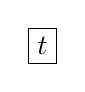
\begin{tikzpicture}
\node[draw]{$t$};
\end{tikzpicture}

We have two choices: 
\begin{enumerate}
\item (terminal production) With probability $p_{t \rightarrow c}$ we
  expand this node to terminal $c$ where $\type{c}$ unifies with $t$,
  and we update the type of the nonterminal to be the most general
  unifier (mgu) of $\type{c}$ and $t$:

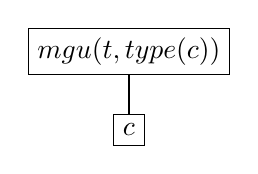
\begin{tikzpicture}
\node[draw](top){$mgu(t, \type{c})$};
\node[draw, below=.5cm of top](c){$c$};

\draw (top)--(c);
\end{tikzpicture}

We propogate this type up the expression tree. If we find a
nonterminal node that can be expanded, we procede with that
expansion. Otherwise, we are done.

\item (nonterminal production) With probability $p_{t \rightarrow
  \epsilon}$ we expand this node into an application:

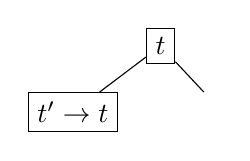
\begin{tikzpicture}
\node[draw](top){$t$};
\node[draw, below left=.5cm of top](left){$\funtype{t'}{t}$};
\node[below right=.5cm of top](right){};

\draw
(top) -- (left)
(top) -- (right);
\end{tikzpicture}
\end{enumerate}


Types:
\begin{grammar}
<$t$> ::= $\tau$, $\sigma$  (type variables)
  \alt $a$, $b$ (concrete types e.g. real, bool, int, etc.)
  \alt $\funtype{t'}{t}$ (function type)
\end{grammar}

Expressions: 
\begin{grammar}
<$\typedexp{e}{t}$> ::= $\typedexp{c}{t'}$ s.t. $t' = mgu(t,
\type{c})$ (substitute a terminal tree that unifies with the requesting type)
  \alt ($\typedexp{e}{\funtype{t'}{t}} \;\;\; \typedexp{e}{t'}$)
\end{grammar}

Let $G(e ; t)$ be the probability of type $t$ yielding expression
$e$. We define $G(\cdot \; ; \cdot)$ according to the following recursion:
\begin{align}
G( (e_1 \;\; e_2 ); t) &\propto \sum_{t' \trianglerighteq t} \phi_{t'} G(e_1 \; ; \; \funtype{s}{t})
   G(e_2 \; ; \;  \text{sourceType}(\type{e_1})\\
G( c \; ; \; t) &\propto \sum_{t' \trianglerighteq t} \phi_{\funtype{t'}{c}}
\end{align}



\section{A nonparametic prior over combinatory expressions}
We would like to describe a distribution over combinatory expressions
such that potential number of ``primitive combinators'' is
unbounded. This will allow us to naturally capture the possibility
that our library of combinator subroutines includes any number of
subroutines (themselves constructed of the primitive combinators). To
do this, we will use a modified version of the Pitman-Yor adaptor
grammar framework~\cite{DBLP:conf/nips/JohnsonGG06}. Our modification
is simply that instead of the base context-free grammar we use the
grammar described in the previous section. 

\section{E-C as MAP inference in a probabilistic graphical model.}
The motivation of the E-C algorithm is that a learning agent should
learn a library of useful program fragments that represents knowledge
about the kind the programs that are likely to solve problems in a
given domain. One way to frame this is as a probabilistic generative
model of the tasks that an agent encounters
(Figure~\ref{fig:generativeModel}).

\begin{figure}
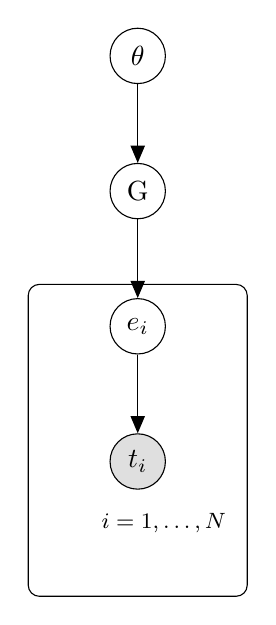
\begin{tikzpicture}[->, circle]

\node[latent] (theta) {$\theta$} ;
\node[latent, below=of theta] (G) {G} ;
\node[latent, below=of G]     (e) {$e_i$} ;
\node[obs, below=of e]     (t) {$t_i$} ;

\edge {theta} {G};
\edge {G} {e};
\edge {e} {t};

\plate {plate} {
  (e)(t)}{$i=1, \dots, N$};

\end{tikzpicture}
\caption{Generative model of program induction
  tasks. \label{fig:generativeModel}}
\end{figure}

Here each task $t_i$ is interpreted as a noisy version of the
underlying program $e_i$, and there is an associated likelihood
function $p_{t|e}(t|e) \propto f(t(e)) $ where $f$ is a monotonically
decreasing function. Given a task-specific loss function $t(\cdot)$, a
natural likelihood is $p_{t|e}(t|e) \propto \exp^{-t(e)}$. A set of
programs $\{e_i\}$ is drawn from a grammar $G$, which functions as the
subroutine library. Our prior expectations about $G$ are encoded in
$\theta$ via the distribution $p_{G|\theta}$. 

The goal of the learner is the find the library $G$ and programs
$\{e_i\}$ that maximize $P(\{e_i\}, G | \{t_i\}, \theta)$. That is, 

\begin{align}
G^*, \{e^*_i\} &= \argmax_{G, \{e_i\} }
   P(\{e_i\}, G | \{t_i\}, \theta)\\
&= \argmax_{G, \{e_i\} } P(\{t_i\} | \{e_i\})
  P(\{e_i\} | G) P(G | \theta)\\
&= \argmax_{G, \{e_i\} }
  \sum_i \left( 
  \log{p_{t|e}(t_i|e_i)}+ 
  \log{p_{e|G}(e_i|G)}
  \right ) +
  \log{p_{G|\theta}(G|\theta)}
\label{eq:objective}
\end{align}

The main difficulty in this optimization is that finding any candidate
program $e_i$ that provides a significant value for the first term is
difficult. If we new $G$, we could sample programs from it as a way to
guide searching over the $e_i$. This suggests the following iterative
heuristic search algorithm. At iteration $j$, let $G^{(j)}$ be the
current best value of $G$. 

\begin{enumerate}
\item \textbf{Exploration step: } Let $F$ be a set of $T$ samples
  i.i.d from $p_{e|G}(\cdot | G^{(j)})$.
\item \textbf{Compression step: } 
$$G^{(j+1)}, \{e^{(j+1)}_i\} = 
\argmax_{G, \{e_i | e_i \in F \}}
\sum_i \left( 
\log{p_{t|e}(t_i|e_i)}+ 
\log{p_{e|G}(e_i|G)}
\right ) +
\log{p_{G|\theta}(G|\theta)}
$$
\end{enumerate}


%% We can break this joint maximization into an iteration of
%% coordinate-wise maximization steps. First we fix $G$ and maximize the
%% programs, then we fix the programs and maximize $G$, repeating until
%% we are no longer improving out objective. This gives us the following
%% iterative algorithm, roughly corresponding to the indicated steps of
%% the E-C algorithm:

%% \begin{enumerate}
%% \item \textbf{Compression step} $$G^{(j+1)} = 
%%   \argmax_{G} \sum_i \left( 
%%   \log{p_{e|G}(e^{(j)}_i|G)}
%%   \right ) +
%%   \log{p_{G|\theta}(G|\theta)}$$
%% \item \textbf{Exploration step} $$\{e^{(j+1)}_i\} = 
%%   \argmax_{\{e_i\}}
%%   \sum_i \left( 
%%   \log{p_{t|e}(t_i|e_i)}+ 
%%   \log{p_{e|G}(e_i|G^{(j)})}
%%   \right ) $$
%% \end{enumerate}









\bibliographystyle{plain} \bibliography{grammar}


\end{document}
